%!TEX encoding = UTF-8 Unicode

%----------------------------------------------------------------------------------------
%   CHAPTER 8
%   translator: laserdog, 日始之音, SI
%   proofreader: SI, lh1962
%----------------------------------------------------------------------------------------
\def\pmm{\begin{pmatrix}}
\def\pmme{\end{pmatrix}}


\chapter[量子力学]{Quantum Mechanics \quad 量子力学}\label{chap8}

{\Huge\bf 总结\\ \ \\}
本章讲述量子力学,基于第\ref{chap5}章讲过的对应关系\footnote{物理量$\to$ 对称性生成元,见\eqref{equ5.1}式。},由此首先可导出{\bf 相对论性能量-动量关系}。

在建立量子力学的基本框架后,我们就对Klein-Gordon方程(最简单的标量型粒子的运动方程)取非相对论极限,得到著名的{\bf Schrödinger方程},方程解被解释为概率幅,随后我们用{\bf 波动力学}的方法分析两个简单例子。

之后呢,我们引入了{\bf Dirac符号},这对于理解量子力学的结构十分有帮助。系统的初始态被一个抽象的态矢量$|i\rangle$标记,称之为{\bf 右矢}。测量该初始态得到某一特定末状态的概率幅可以用左矢(记作$\langle f|$,表示末态)乘以右矢$|i \rangle$计算。左矢与右矢的乘积$\langle f | i \rangle$是一个复数,即为状态$i \to f$的概率幅,发生这个过程的概率就是$|A|^2$。之后讨论{\bf 投影算符}。我们会看到它是如何与{\bf 完备性关系}一起用来把任意状态用任意一个算符的本征态来进行展开的。之前常用的波动力学方法可以视为将态矢在坐标基底展开的特例。在Dirac符号下,Schrödinger方程用来计算态的时间演化。为了阐明这一联系,我们会用Dirac符号来重新讨论一个前面用波动力学求解过的例子。

\section[对应到粒子理论]{Particle Theory Identifications \quad 对应到粒子理论}\label{sec8.1}
前面导出的方程\mpar{Klein-Gordon, Dirac, Proka, Maxwell方程}可以用在粒子理论和场理论中。本章考虑它们应用于粒子理论的情形。因此动力学变量就是粒子(们)的坐标、能量和动量。第\ref{chap5}章讲过,这些物理量可视为相应对称性的生成元:\mpar{见\eqref{equ3.240},\eqref{equ3.244}和第\ref{chap5}章。}
\begin{itemize}
\item 动量$\hat{p}_i=-i\partial_i$\\
\item 坐标$\hat{x}_i=x_i$\\
\item 能量$\hat{E}=i\partial_0$\\
\item 角动量$\hat{L}_i=i\frac{1}{2}\epsilon_{ijk}(x^j\partial^k-x^k\partial^j)$
\end{itemize}

在讨论这些算符是如何应用于量子力学之前,我们先用它们导出现代物理最重要的方程之一。
\section[相对论性能量-动量关系]{Relativistic Energy-Momentum Relation \quad 相对论性能量-动量关系}\label{sec8.2}
第\ref{sec6.2}节推导了自旋$0$自由场的运动方程——Klein-Gordon方程:
\[(\partial_\mu\partial^\mu+m^2)\Phi=0, \]

利用上一节的那些对应关系\mpar{$p_\mu=\left(\begin{matrix}p_0\\p_1\\p_2\\p_3\end{matrix}\right)=\left(\begin{matrix}p_0\\\vec{p}\end{matrix}\right)=\left(\begin{matrix}E\\\vec{p}\end{matrix}\right)$},
\begin{align}
  (\partial_\mu\partial^\mu+m^2)\Phi&=(\partial_0\partial_0-\partial_i\partial_i+m^2)\Phi \notag \\
  &=\left(\left(\frac{1}{i}E\right)\left(\frac{1}{i}E\right)-\left(-\frac{1}{i}p_i\right)\left(-\frac{1}{i}p_i\right)+m^2\right)\Phi \notag \\
\label{equ8.1}
  &=(-E^2+\vec{p}^{\,2}+m^2)\Phi=0 \\
\label{equ8.2}
  \to\ E^2=\vec{p}^{\,2}+m^2 & \quad\text{ 或者用4-矢量表示:}p_\mu p^\mu=m^2
\end{align}
这就是著名的狭义相对论{\bf 能量-动量关系}。上式应用于静止粒子($\vec{p} = 0$)即得到Einstein著名的质能方程:
\[E^2=m^2\to E=mc^2 \]
其中为了明确起见我们把$c^2$写回来。现在就理解了Poincare群的第一个Casimir算符$p_\mu p^\mu$的标量值(见\eqref{equ3.258}式)为何选为$m^2$了。$p_\mu p^\mu$就代表着粒子质量的平方,而通过实验,比如说测量粒子的能量和动量,就可测量质量$m=\sqrt{E^2-\vec{p}^{\,2}}$。同理,我们也可以理解为什么\ref{sec6.2}节要把拉格朗日量里面的系数常数记作$m^2$。

\section[量子力学的数学形式]{The Quantum Formalism\quad 量子力学的数学形式}
\label{sec8.3}

前面说过,物理量用算符表示,这些算符作用于什么对象?首先需要注意每个算符都有一组本征函数,就像矩阵的本征向量一样。矩阵是有限维的,因此矩阵有有限多个本征向量;而算符通常作用在无限维的矢量空间中,而得到无穷多个本征函数。比如,动量算符的本征函数满足的本征方程为
\begin{align}
\label{equ8.3}
	\underbrace{-i\partial_i\Psi}_{\mathclap{\text{算符}}}=\underbrace{p_i}_{\mathclap{\text{本征值}}}\overbrace{\Psi}^{\mathclap{\text{本征函数}}}
\end{align}
其中,$p_i$是一个数。一个显然的解为
\begin{align}
	&\underbrace{C}_{\mathclap{=\text{常数}}}e^{ip_ix_i} \notag \\
\label{equ8.4}
	&\to-i\partial_iCe^{ip_ix_i}=p_iCe^{ip_ix_i}\checkmark
\end{align}
但要注意,对于任意的$p_i$,这都是一个解。因此我们发现有无穷多个动量算符$\hat{p}_i=-i\partial_i$的本征函数。能量本征函数同理
\begin{align}
i\partial_0\Phi=E\Phi
\end{align}
或者角动量的本征函数\mpar{角动量本征函数的求解更加复杂,因为角动量算符比其它算符本身就更复杂。我们找不到一组三个角动量分量共同的本征态,因为$[\hat{L}_i,\hat{L}_j]\neq0$。这在后面就会详细讨论,最终选取的本征函数是角动量第三个方向$\hat{L}_3$(和角动量算符的平方$\hat{L}^2$,它与其它的角动量分量都对易$[\hat{L}^2,\hat{L}_j]=0$)的完备归一基,即著名的{\bf 球谐函数基}。}。类比于矩阵的本征矢量,这些本征函数可以看做基\mpar{在矩阵中,本征矢量是矩阵对应的矢量空间的基},而这就意味着我们可以把任意的函数$\Psi$按照这些基进行展开。例如,在动量本征函数\mpar{注意,这其实就是我们在附录\ref{appendix.D.1}中介绍的Fourier变换,因子$\frac{1}{\sqrt{2\pi}}$是出于惯例的考虑。}进行展开(简明起见,考虑一维情形)
\begin{align}
\label{equ8.6}
	\Psi=\frac{1}{\sqrt{2\pi}}\int_{-\infty}^\infty dp\Psi_pe^{-ipx}
\end{align}
其中,$\Psi_p$是展开系数,类似于矢量$\vec{v}=v_1\vec{e}_1+v_2\vec{e}_2+v_3\vec{e}_3$中的$v_1,v_2,v_3$。对于一些系统来说,我们的边界条件使得最后得到的基是离散而不连续的。我们可以,比如说,用能量本征态$\Phi_{E_c}$进行展开:
\begin{align}
\label{equ8.7}
	\Psi=\sum_n c_n\Phi_{E_n}
\end{align}
注意,一般来说,一个算符的本征函数并不是另一个算符的本征函数。只有当两个算符对易,即$[A,B]=AB-BA=0$时,才可以找到一组同时是两个算符本征函数的基。下面证明这个命题。设$[C,D]\neq0\to CD\neq DC$,而对于$C$的某个本征函数$\Psi$,有$C\Psi=c\Psi$,其中$c$是它的本征值。如果$\Psi$同时也是$D$的本征函数$D\Psi=d\Psi$,则有
\[CD\Psi=Cd\Psi\underbrace{=}_{\mathclap{\text{因为$d$只是一个数}}}dC\Psi=dc\Psi \]
\[DC\Psi=Dc\Psi=cD\Psi=cd\Psi\underbrace{=}_{\mathclap{\text{因为数之间互相对易}}}dc\Psi \]
\begin{align}
\label{equ8.8}
	\to DC=CD\quad \text{这与$[C,D]\neq0$矛盾,因而不存在共同的本征函数。}
\end{align}

一般来说,物理量算符作用在描述物理系统的{\bf 态}\mpar{这里使用$\Psi$是出于量子力学的惯例,尽管前面只用它表示描述自旋$0$粒子的旋量。}$\Psi$上,通过求解运动方程得到$\Psi$。

一般的解按照某组基展开都会超过一项。举个例子,考虑两个能量本征态\footnote{即能量算符(蛤密顿算符)$\hat{H}$的本征态,能量本征值为$E$的本征态记作$\Phi_E$.}$\Psi = c_1 \Phi_{E_1} + c_2 \Phi_{E_2}$\mpar{这意味着所有的展开系数$\Psi=\sum_nc_n\Phi_{E_n}$是零。},能量算符作用于它可得
\begin{align}
\label{equ8.9}
	\hat{E}\Psi = \hat{E}(c_1\Phi_{E_1} + c_2\Phi_{E_2})=c_1E_1\Phi_{E_1}+c_2E_2\Phi_{E_2}\neq E(c_1\Phi_{E_1}+c_2\Phi_{E_2})
\end{align}
由此可见不同能量(的能量本征态)形成的{\bf 叠加态}一般不是能量算符的本征态,因为本征态需要满足定义——存在某个数$E$使得$\hat{E}\Psi=E\Psi$。不过,处于$\Psi$状态系统的能量是多少呢?两个能量本征态的叠加态又意味着什么呢?它的物理意义是什么?

首先我们能从拉格朗日量的$\mathcal{U}(1)$对称性中得到一点提示,它表明从$\Psi$的运动方程得到的解没有直接的物理意义\mpar{如果假定$\Psi$直接描述粒子,那么它的$\mathcal{U}(1)$变换$\Psi'=e^{i\alpha}\Psi$(也是运动方程的解)描述的是什么呢?}。

另一方面,注意到运动方程所有的解都是$\vec{x},t$的函数\mpar{下一节会对这点详细说明。},即$\Psi=\Psi(\vec{x},t)$。

标准的诠释是,{\bf 波函数}$\Psi(\vec{x},t)$模长的平方$|\Psi(\vec{x},t)|^2$表示粒子位置的概率密度。注意$\mathcal{U}(1)$变换对于$|\Psi|^2=\Psi^\dagger\Psi\to(\Psi')^\dagger(\Psi')=\Psi^\dagger e^{-i\alpha}e^{i\alpha}\Psi=\Psi^\dagger\Psi$这样的量是没有影响的。换句话说(以一维情形为例),$\Psi(x,t)$是在$[x, x+dx]$区间内测量到粒子的概率密度\footnote{即在区间$[x, x + dx]$测量到粒子的概率为$|\Psi(x, t)|^2 dx$.}。因此,如果对整个空间积分的话,必定有
\begin{align}
\label{equ8.10}
	\int dx\Psi^*(x,t)\Psi(x,t)\overset{!}{=}1
\end{align}
这称为波函数的归一化,因为在全空间中找到一个粒子的概率必定为$100\%=1$。

如果要预言其他物理量,则必须把波函数用相应的本征函数基展开。比如说用能量本征基展开:$\Psi=c_1\Phi_{E_1}+c_2\Phi_{E_2}+\cdots$。标准的量子力学诠释是,测量$\Psi$状态的体系的能量,所得结果只能为能量本征值,测量结果为本征值$E_1$的概率为$\Psi$与能量本征函数$\Phi_{E_1}$的“交叠”(的绝对值平方):
\[P(E_1)=\left|\int dx\Phi^*_{E_1}(x,t)\Psi(x,t)\right|^2 \]
在上面的例子中,它就是
\begin{align}
\label{equ8.11}
	\begin{split}
	P(E_1)&=\left|\int dx\Phi^*_{E_1}(x,t)\Psi(x,t)\right|^2 =\left|\int dx\Phi^*_{E_1}(x,t)(c_1\Phi_{E_1}+c_2\Phi_{E_2}+\cdots)\right|^2 \\
	&=\left|c_1\underbrace{\int dx\Phi^*_{E_1}(x,t)\Phi_{E_1}}_{=1\text{ 如之前所讲}}+\underbrace{\int dx\Phi^*_{E_1}(x,t) (c_2\Phi_{E_2}+\cdots)}_{\mathclap{=0\text{ 因为本征态是正交的}}}\right|^2\\
	&=|c_1|^2
	\end{split}
\end{align}
类似的,可以将$\Psi(\vec{x}, t)$用动量本征函数展开:
\[\Psi(\vec{x},t)=\frac{1}{\sqrt{2\pi}}\int_{-\infty}^{\infty}d^3 p\Psi(\vec{p},t)e^{-i\vec{p}\cdot\vec{x}}, \]
则$\Psi(\vec{p},t)$是系统动量处于$[p,p+dp]$区间内的概率幅。

这种解释可以用来对系统做几率性预测,比如用下一节介绍的统计期望值的办法。之后我们会导出非相对论性量子力学的运动方程,并看两个例子。

\subsection[期望值]{Expectation Value \quad 期望值}\label{sec8.3.1}

统计学中,期望值是类比于加权平均定义的。比如,如果掷骰子十次得到的结果为$2,4,1,3,3,6,3,1,4,5$,那么它的平均值就是
\[\langle x \rangle = (2+4+1+3+3+6+3+1+4+5)\cdot\frac{1}{10}=3.2 \]
而另一种计算这个的方法是计算每种相同结果的权重,给出经验几率
\[\langle x \rangle = \frac{2}{10}\cdot1+\frac{1}{10}\cdot2+\frac{3}{10}\cdot3+\frac{2}{10}\cdot4+\frac{1}{10}\cdot5+\frac{1}{10}\cdot6=3.2 \]
一般的,我们可以写
\begin{align}
\label{equ8.12}
	\langle x\rangle = \sum_i\rho_i x_i
\end{align}
其中$\rho_i$表示几率。对一个连续分布的情况同样有
\begin{align}
\label{equ8.13}
	\langle x\rangle = \int dx\rho(x)x
\end{align}

类比上面的形式,在量子力学中物理量$\hat{\mathcal{O}}$期望值的定义为
\begin{align}
\label{equ8.14}
	\langle \hat{\mathcal{O}}\rangle = \int d^3x\Psi^*\hat{\mathcal{O}}\Psi
\end{align}
一般的,要把$\Psi$按照$\hat{\mathcal{O}}$的本征函数展开,比如说动量本征函数。然后,把算符$\hat{\mathcal{O}}$作用在这些态上,得到对应的本征值,这样就得到了加权和。

举个例子,处于$\Psi$态的粒子的坐标期望值为
\begin{align}
\label{equ1.15}
	\langle \hat{x}\rangle = \int d^3x\Psi^*\hat{x}\Psi= \int d^3x\Psi^*{x}\Psi= \int d^3x\, x\underbrace{\Psi^*\Psi}_{\mathclap{\text{在位置}x\text{的几率密度}}}
\end{align}

为了计算方便,下面取Klein-Gordon方程的非相对论极限。


\section[Schrödinger 方程]{Schrödinger Equation \quad Schrödinger 方程}\label{sec8.4}
Klein-Gordon方程有平面波解
\[\Phi = \mathrm{e}^{\pm ip_\mu x^\mu} \equiv \mathrm{e}^{\pm ip\cdot x} \]
其中,$p_\mu=(E,\vec{p})^T$,是粒子四动量(满足守恒律):
\begin{align}
	0&=(\partial_\mu\partial^\mu+m^2)\Phi \notag \\
	&=(\partial_\mu\partial^\mu+m^2) \mathrm{e}^{\pm ip_\mu x^\mu} \notag \\
	&=(i^2 p_\mu p^\mu+m^2) \mathrm{e}^{\pm ip_\mu x^\mu}=0 \notag \\
\label{equ8.16}
	&=(-m^2+m^2) \mathrm{e}^{\pm ip_\mu x^\mu}=0\quad \checkmark
\end{align}

我们可以把解写成稍不同的形式
\[\Phi = \mathrm{e}^{\pm ip_\mu x^\mu}=\Phi= \mathrm{e}^{i(-Et+\vec{x}\cdot\vec{p})} \]
$\Phi$的时间部分是$\mathrm{e}^{-iEt}$,即$\Phi\propto \mathrm{e}^{-iEt}$。从\eqref{equ8.2}式可知
\[E=\sqrt{\vec{p}^2+m^2}=\sqrt{m^2\left(\frac{\vec{p}^2}{m^2}+1\right)}=m\sqrt{\frac{\vec{p}^2}{m^2}+1}. \]
在非相对论极限$|\vec{p}|\ll m$下,即研究对象的移动速度比光速要慢很多,从而其动量比质量也要小很多的情形下,可以对能量进行Taylor展开:
\[\begin{split}
E&=m\left(1+\frac{1}{2}\frac{\vec{p}^2}{m^2}+\cdots\right)\\
&\to E\approx\underbrace{m}_{\mathclap{\text{静质量}}}+\underbrace{\frac{\vec{p}^2}{2m}}_{\mathclap{\text{动能}}}.
\end{split} \]
于是
\begin{align}
\label{equ8.17}
	\Phi=\mathrm{e}^{i(-Et+\vec{x}\cdot\vec{p})}\approx \mathrm{e}^{-imt}\underbrace{\mathrm{e}^{i\vec{p}\cdot\vec{x}-i(p^2/2m)t}}_{\equiv\phi(\vec{x},t)}=\mathrm{e}^{-imt}\phi(\vec{x},t)
\end{align}

由$|\vec{p}|\ll m$可知静质能远大于粒子动能,因此$\phi(\vec{x}, t)$的振动频率远低于$\mathrm{e}^{-imt}$. 把$\mathrm{e}^{-imt}\phi(\vec{x},t)$作为试探解\footnote{译者注:ansatz是个很奇怪的词,我不知道怎么翻译。。比如Bethe-Ansatz,叫Bethe近似嘛也不对,叫啥都不对。}带入Klein-Gordon方程可得\footnote{原文下式有误,译文已按照勘误表改正。}
\[(\partial_\mu\partial^\mu+m^2) \mathrm{e}^{-imt}\phi(\vec{x},t)=(\partial_0\partial^0 - \partial_i\partial^i+m^2) \mathrm{e}^{-imt}\phi(\vec{x},t)=0. \]
根据莱布尼兹律,$\partial_t \mathrm{e}^{-imt}(\dots)= \mathrm{e}^{-imt}(-im+\partial_t)(\dots)$,即简单的把微分算符作用出来,我们得到
\[\mathrm{e}^{-imt} \big( (-im + \partial_t)^2 + \partial_i\partial^i + m^2 \big) \phi(\vec{x},t) = 0, \]
两边可以除掉$\mathrm{e}^{-imt}$,因为它肯定不是零。因此,
\[\begin{split}
\to \big((-im+\partial_t)^2+\nabla^2+m^2 \big)\phi(\vec{x},t)=0\\
\to \big( -m^2 - 2im\partial_t + (\partial_t)^2 + \nabla^2 + m^2 \big) \phi(\vec{x},t)=0.
\end{split} \]
把第三项
\begin{align}
	(\partial_t)^2 \phi(\vec{x},t) &= (\partial_t)^2 \exp\big[i\vec{p}\cdot\vec{x}-i(\vec{p}^2/2m)t \big] \notag \\
\label{equ8.18}
	&= \left(\frac{\vec{p}^2}{2m}\right)^2 \exp\big[ i\vec{p}\cdot\vec{x} - i(\vec{p}^2/2m)t \big] \propto\frac{p^4}{m^2}.
\end{align}
与第二项对比
\begin{align}
	im\partial_t\phi(\vec{x},t) &= im\partial_t\exp \big[i\vec{p}\cdot\vec{x} - i(\vec{p}^2/2m)t \big] \notag \\
\label{equ8.19}
	&= m \left( \frac{\vec{p}^2}{2m} \right) \exp\big[i\vec{p}\cdot\vec{x}-i(\vec{p}^2/2m)t \big] \propto p^2.
\end{align}
这表明,在$|\vec{p}|\ll m$的极限下,第三项可忽略,因此\footnote{原文下式有误,译文已按勘误表修改}
\begin{align}
	(-2im\partial_t+\nabla^2)\phi(\vec{x},t)=0 \notag \\
	\underbrace{\to}_{\mathclap{\text{除以}(-2m)}}\left(i\partial_t-\frac{1}{2m}\nabla^2\right)\phi(\vec{x},t)=0 \notag \\
\label{equ8.20}
	\to \left( i \partial_t + \frac{\nabla^2}{2m} \right) \phi(\vec{x}, t) = 0,
\end{align}
这就是著名的{\bf Schrödinger 方程}。利用本章开头物理量与算符的对应关系,Schrödinger方程写为\footnote{原文下式有误,译文已按勘误表修改}
\begin{align}
	& \to \bigg( E - \underbrace{\frac{\vec{p}^2}{2m} }_{=\text{动能}} \bigg) \phi (\vec{x}, t) = 0  \notag \\
\label{equ8.21}
	& \to E = \frac{\vec{p}^2}{2m}.
\end{align}
此即为{\bf 非相对论性能量—动量关系}。

从该式出发很容易考虑粒子位于外势场$V$中的情况,因为外势场中粒子的能量就是动能加势能:
\[
	\to E = \frac{\vec{p}^2}{2m} + V.
\]
典型的例子有谐振子势$V = -k x^2$. Schrödinger方程通常用所有能量算符的总和(例如动能\footnote{\textcolor{red}{译注:原文缺负号,已更正。}}$-\frac{\nabla^2}{2m}$加势能$\hat{V}$)——蛤密顿算符$\hat{H}$表示,即:
\begin{align}
	i \partial_t \phi(\vec{x}, t) = \underbrace{-\frac{\nabla^2}{2m} }_{\equiv \hat{H}} \phi(\vec{x}, t) \notag \\
\label{equ8.22}
	\to i \partial_t \phi(\vec{x}, t) = \hat{H} \phi(\vec{x}, t).
\end{align}
Dirac方程的非相对论极限的计算过程类似,所得结果称为Pauli方程。



\subsection[有外场的 Schr\"{o}dinger 方程]{Schr\"{o}dinger Equation with External Field 有外场的 Schr\"{o}dinger 方程}\label{sec8.4.1}

此外,我们可以对{\bf 相互作用}Klein-Gordon方程\eqref{equ7.43}式,即描述有质量的$0$自旋场与无质量的自旋$1$场(光子场)相互作用的方程,做同样的非相对论性近似。所得结果为
\begin{align}
\label{equ8.23}
	\left(i\partial_t+\frac{1}{2m}\left(\nabla-ia\vec{A}\right)^2+q\Phi\right)\phi(\vec{x},t)=0
\end{align}

\section[从波动方程到粒子的运动]{From Wave Equations to Particle Motion \quad 从波动方程到粒子的运动}\label{sec8.5}
本节讨论量子力学标准诠释的两个典型例子。

\subsection[例:自由粒子]{Example: Free Particle \quad 例:自由粒子}\label{sec8.5.1}
自由粒子(无外部势场)Schrödinger方程\eqref{equ8.20}式的一个特解(称为平面波解)为:
\begin{equation}
\label{equ8.24}
	\Psi = \mathrm{e}^{-i (Et - \vec{p} \cdot \vec{x})},
\end{equation}
验证:
\begin{align}
	i \partial_t \mathrm{e}^{-i (Et - \vec{p} \cdot \vec{x}) } &= -\frac{\nabla^2}{2m} \mathrm{e}^{-i (Et - \vec{p} \cdot \vec{x}) } \notag \\
\label{equ8.25}
	\to E \mathrm{e}^{-i(Et - \vec{p} \cdot \vec{x}) } &= \frac{\vec{p}^2}{2m} \mathrm{e}^{-i(Et - \vec{p} \cdot \vec{x}) }.
\end{align}
其中$E$是自由粒子总能量的值,$E = \frac{\vec{p}^2}{2m}$(\eqref{equ8.21}式)。各特解的线性组合为更一般的解:
\[ \Psi = A \mathrm{e}^{-i(Et - \vec{p} \cdot \vec{x}) } + B \mathrm{e}^{-i (E' t + \vec{p}' \cdot \vec{x}) } + \dots . \]

	\marginpar{
		\centering
		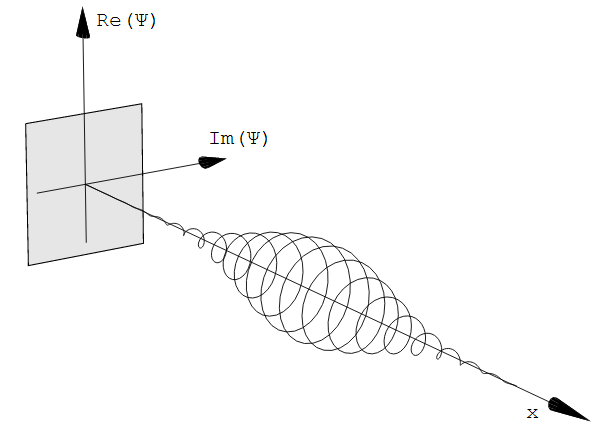
\includegraphics[width = 5cm]{./../Pictures/fig8_1.png}
		\figcaption{自由高斯波包图示。 Figure by Inductiveload (Wikimedia Commons) released under
		a public domain license. URL: \url{https://upload.wikimedia.org/wikipedia/commons/4/49/Travelling_Particle_Wavepacket.svg}}}

波函数$\Psi$被诠释为概率幅,因此描述真实粒子的波函数必定是归一化的,因为在粒子在全空间的概率为$100\% = 1$. 上面的波函数不能归一化,它散布在全空间。因此采用平面波的合适的线性组合(称为波包(wave-packet))来描述一个真实的自由粒子:
\begin{equation}
\label{equ8.26}
	\Psi_{WP} (\vec{x}, t) = \int d^3 p A(\vec{p}) \mathrm{e}^{i (\vec{p} \cdot \vec{x} - Et)},
\end{equation}
其中系数$A(\vec{p})$为复数,由归一化条件求出。典型的波包是高斯波包,它的$A(\vec{p})$服从高斯分布:
\[
	\Psi_{GWP} = \int d^3 p\, A(\vec{p}) \mathrm{e}^{i (\vec{p} \cdot \vec{x} - Et)} = \int d^3 p\, \psi_0 \mathrm{e}^{i (\vec{p} - \vec{\tilde{p}})^2 / 4\sigma^2} \mathrm{e}^{i (\vec{p} \cdot \vec{x} - Et)}.
\]
其中$\vec{\tilde{p}}$为常数向量。

典型的高斯波包如图8.1. 在实际计算中经常采用特殊技巧避免求解复杂波包,而是处理更简单的波函数。

\subsection[例:盒子中的粒子]{Example: Particle in a Box \quad 例:盒子中的粒子}\label{sec8.5.2}
	\marginpar{
		\centering
		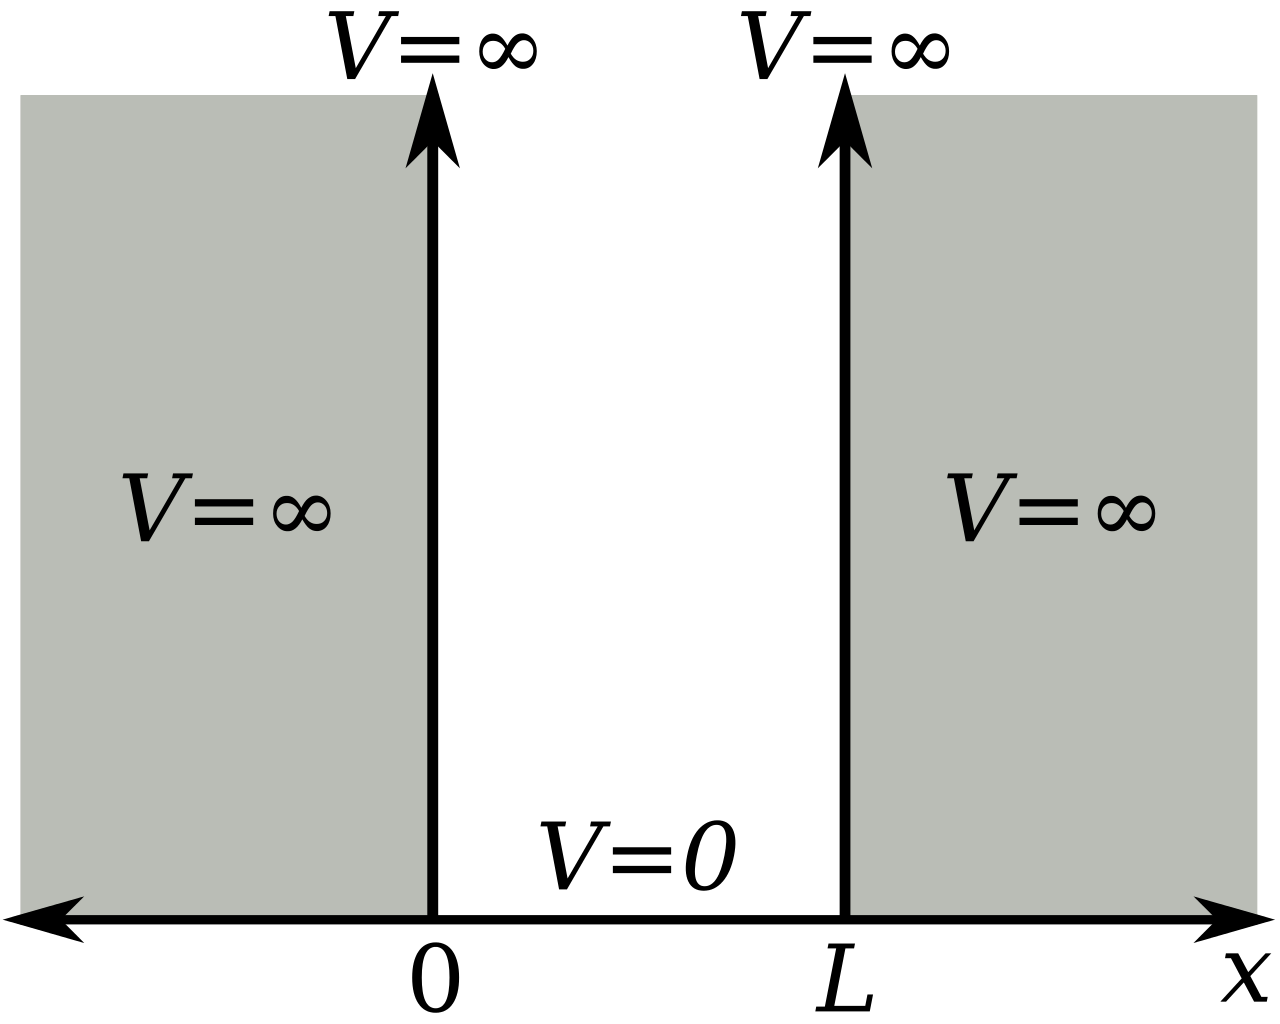
\includegraphics[width = 4.2cm]{./../Pictures/fig8_2.png}
		\figcaption{一维无限深势阱(硬盒)。  Figure by Benjamin D. Esham (Wikimedia Commons) released under a public domain licence. URL: \url{https://upload.wikimedia.org/wikipedia/commons/2/27/Infinite_potential_well.svg}, Accessed: 4.5.2014 }
	}

下面讨论量子力学的标准例子\footnote{几乎任何一本量子力学教材都会有吧……}:一个粒子被限制在一维的、势垒无限高的硬盒内,即,盒子内的势能为零,盒外的势能为无穷大,如图8.2.

无限深势阱数学上用一个分段函数表示:
\begin{equation}
\label{equ8.27}
	V =
		\begin{cases}
			0, & 0 < x < L, \\
			\infty, & \text{其它}.
		\end{cases}
\end{equation}
因此需要分段求解Schrödinger方程
\[
	i \partial_t \Psi(\vec{x}, t) = -\frac{1}{2m} \partial_x^2 \Psi(x, t) + V(x) \Psi(x, t).
\]
\begin{itemize}
	\item 势阱内$V = 0, 0 < x < L$,方程的解即为自由粒子波函数。
	\item 势阱外$V = \infty$,具有物理意义的解仅有$\Psi(x, t) = 0$,即由于势垒无穷大,粒子不可能在势阱外出现。
\end{itemize}

将自由粒子波函数的一般形式写为\mpar{下式利用了$\sin x = \frac{1}{2i} (\mathrm{e}^{ix} - \mathrm{e}^{-ix}$以及$\cos x = \frac{1}{2} (\mathrm{e}^{ix} + \mathrm{e}^{-ix})$, 这两个式子可以从$\cos x, \sin x, \mathrm{e}^{ix}$的级数展开式导出,详见附录B.4.1.}:
\begin{align*}
	\Psi (x, t) &= A \mathrm{e}^{-i (Et - \vec{p} \cdot \vec{x})} + B \mathrm{e}^{-i (Et + \vec{p} \cdot \vec{x})} \\
	&= \Big( C \sin (\vec{p} \cdot \vec{x}) + D \cos (\vec{p} \cdot \vec{x}) \Big) \mathrm{e}^{-iEt},
\end{align*}
利用\eqref{equ8.21}式表示的非相对论能量-动量关系,上式写为:
\begin{align}
	E &= \frac{\vec{p}^2}{2m} \to |\vec{p}| = \sqrt{2mE} \notag \\
\label{equ8.28}
	\Psi (x, t) &= \Big( C \sin (\sqrt{2mE} x) + D \cos (\sqrt{2mE} x) \Big) \mathrm{e}^{-iEt}
\end{align}
利用波函数的连续性\mpar{如果波函数在某处不连续,则粒子动量$\hat{p}_x \Psi = -i\partial_x \Psi$为无穷大(跃变点处的导数无穷大),不符合基本法。}可得边界条件为$Psi(0) = \Psi(L) \stackrel{!}{=} 0.$ 带入上式,由于$\cos 0 = 1$故而$D \stackrel{!}{=} 0$. 此外还有
\begin{equation}
\label{equ8.29}
	\sqrt{2mE} \stackrel{!}{=} \frac{n\pi}{L}, \quad n = 1, 2, 3, \dots
\end{equation}
于是满足边界条件的波函数为\mpar{注意下面给波函数添加了编号$n$,因为由上式可见每个$n$都对应一个解。}:
\begin{equation}
\label{equ8.30}
	\Phi_n (x, t) = C \sin \left( \frac{n \pi}{L} x \right) \mathrm{e}^{-i E_n t}.
\end{equation}
验证:
\begin{align*}
	\to \Phi_n (L, t) &= C \sin \left( \frac{n\pi}{L} L \right) \mathrm{e}^{-i E_n t} = C \sin(n \pi) \mathrm{e}^{-i E_n t} = 0 \quad \checkmark \\
	\to \Phi_n (0, t) &= C \sin \left( \frac{n\pi}{L} 0 \right) \mathrm{e}^{-i E_n t} = C \sin (0) \mathrm{e}^{-i E_n t} = 0 \quad \checkmark
\end{align*}
不难求出归一化常数$C = \sqrt{ \frac{2}{L} }$,注意在盒内($0 < x < L$)找到粒子的概率为$100 \% = 1$,而盒外的概率为零:
\begin{align*}
	P &= \int_0^L dx\, \Phi^*_n (x, t) \Phi_n (x, t) \stackrel{!}{=} 1 \\
	P &= \int_0^L dx\, C^2 \sin \left( \frac{n \pi}{L} x \right) \mathrm{e}^{+iEt} \sin \left( \frac{n \pi}{L} x \right) \mathrm{e}^{-iEt} \\
	&= C^2 \int_0^L dx\, \sin^2 \left( \frac{n \pi}{L} x \right) = C^2 \left[ \frac{x}{2} - \frac{ \sin\big( \frac{2n\pi}{L} x \big) }{ 4 \frac{n \pi}{L} } \right]_0^L \\
	&= C^2 \left( \frac{L}{2} - \frac{ \sin \left(\frac{2n\pi}{L} L \right) }{ 4 \frac{n \pi}{L} } \right) = C^2 \frac{L}{2} \stackrel{!}{=} 1 \\
	\to C^2 &\stackrel{!}{=} \frac{2}{L} \quad \checkmark
\end{align*}
解\eqref{equ8.29}式得到盒中粒子的能级为
\begin{equation}
\label{equ8.31}
	E_n \stackrel{!}{=} \frac{n^2 \pi^2}{L^2 2m}.
\end{equation}
{\bf 粒子可能具有的能量是量子化的},即能量只能是某个常量(这里是$\frac{\pi^2}{L^2 2m}$)的整数倍,这就是量子力学名字的来历。

每个$n$都对应一个解,解的线性组合
\[
	\Phi (x, t) = A \Phi_1 (x, t) + B \Phi_2 (x, t) + \dots
\]
仍然是Schrödinger方程的解。各线性系数$A, B, \dots$要满足归一化条件\mpar{大于$1 = 100\%$的概率没有意义。}。

下面考虑能量的问题\mpar{前面讨论的是粒子位置的概率分布。},例如,测量一个(归一化的)状态为
\[
	\Psi (x, t) = \sqrt{\frac{3}{5}} \Phi_2 (x, t) + \sqrt{\frac{2}{5}} \Phi_3 (x, t).
\]
的粒子,测得能量$E = E_2 = \frac{2^2 \pi^2}{L^2 2m}$的概率是多少?

量子力学经典诠释给出的答案是:概率$P (E = E_2)$等于粒子状态$\Psi$与$E_2$对应的本征态$\Phi_2$“重叠”绝对值的平方:
\[
	P ( E = \frac{2^2 \pi^2}{L^2 2m} ) = \left| \int dx\, \Phi_2^* (x, t) \Psi (x, t) \right|^2.
\]
$\Phi_2$与$\Psi$的重叠可以视为它们的标量积\mpar{实际上,$\Psi, \Phi_n$是Hilbert空间的向量,$(\Psi, \Phi_n)$正是它们的标量积。}:
\[
	(\Phi_2, \Psi) = \int dx\, \Phi_2^* \Psi = \underbrace{c}_{\mathclap{\text{复数}} }.
\]
上述积分可以利用本征状态的正交归一性大大简化计算
\[
	\int dx\, \Phi_n^* (x, t) \Phi_{n'} (x, t) = \delta_{n n'}
\]
例如\mpar{不难用分部积分或者Wolframalpha检验计算结果。}:
\begin{align*}
	\int_0^L dx\, \Phi_2^* \Phi_3 (x, t) &= \int_0^L dx\, C \sin \left( \frac{2\pi}{L} x \right) \mathrm{e}^{+iEt} C \sin \left( \frac{3\pi}{L} x \right) \mathrm{e}^{-iEt} \\
	&= C^2 \int_0^L dx\, \sin \left( \frac{2\pi}{L} x \right) \sin \left( \frac{3\pi}{L} x \right) = 0.
\end{align*}
因此测量得到能量$E = \frac{2^2 \pi^2}{L^2 2m}$的概率为
\begin{align}
	P ( E = \frac{2^2 \pi^2}{L^2 2m} ) &= \left| \int dx\, \Phi_2^* (x, t) \Psi(x, t) \right|^2 \notag \\
	&= \left| \int dx\, \Phi_2^* (x, t) \left( \sqrt{\frac{3}{5}} \Phi_2 (x, t) + \sqrt{\frac{2}{5}} \Phi_3 (x, t) \right) \right|^2 \notag \\
	&= \left| \int dx\, \left( \sqrt{\frac{3}{5}} \underbrace{ \Phi_2^* (x, t) \Phi_2 (x, t) }_{ \text{积分后等于}1 } + \sqrt{\frac{2}{5}} \underbrace{ \Phi_2^* (x, t) \Phi_3(x, t) }_{ \text{积分后等于}0 } \right) \right|^2 \notag \\
\label{equ8.32}
	&= \left( \sqrt{\frac{3}{5}} \right)^2.
\end{align}

\eqref{equ8.30}式的波函数解称为能量算符$i \partial_t$的本征态,或者蛤密顿算符\mpar{这可以从Schrödinger方程直接导出:\[ i\partial_t \Phi = -\frac{\partial^2_x}{2m} \Phi \equiv \hat{H} \Phi. \]} $\hat{H} \equiv -\frac{\partial^2_x}{2m}$的本征态,因为
\begin{equation}
\label{equ8.33}
	\hat{H} \Phi_n = E_n \Phi_n.
\end{equation}
能量算符作用于能量本征态得到的结果为该本征态的常数倍,这个常数即为该状态的能量。注意能量算符(或蛤密顿算符)作用于一般状态造成的变化不止变成常数倍这么简单。例如,考虑如下能量本征态的线性组合:
\[
	\Psi = \sqrt{\frac{3}{5}} \Phi_2 + \sqrt{\frac{2}{5}} \Phi_3.
\]
蛤密顿算符作用其上得到:
\[
	\hat{H} \Psi = \hat{H} \left( \sqrt{\frac{3}{5}} \Phi_2 + \sqrt{\frac{2}{5}} \Phi_3 \right) \underbrace{=}_{\mathclap{ \eqref{equ8.33}\text{式}} } \sqrt{\frac{3}{5}} E_2 \Phi_1 + \sqrt{\frac{2}{5}} E_3 \Phi_3.
\]
作用后的结果不能再写成$\Psi$的常数倍了,因为$E_2 \neq E_3$. 因此$\Psi$不是能量算符的本征态。然而$\Psi$可以表示为各$\Phi_n$的线性组合,因为能量本征态$\{ \Phi_n \}$构成一组完备基。

下一节介绍由Dirac发明的十分便捷的Dirac符号,它有助于我们理解量子力学的框架结构。

\subsection[Dirac符号]{Dirac Notation \quad Dirac符号}\label{sec8.5.3}
Dirac符号中,系统状态由{\bf 右矢 (ket)}\mpar{它的含义稍后会进一步说明。}表示,记作
\begin{equation}
\label{equ8.34}
	|\Psi \rangle,
\end{equation}
例如,一个硬盒中的状态为$\Phi_n$的粒子的能量本征方程用Dirac符号写为
\[
	\hat{H} |\Phi_n \rangle = E_n |\Phi_n \rangle.
\]
每个右矢可以定义相应的{\bf 左矢 (bra)},记作$\langle \Psi|$,定义为
\begin{equation}
\label{equ8.35}
	\langle \Psi|^\dag = |\Psi \rangle,
\end{equation}
其中符号$\dag$表示厄米共轭,即转置+复共轭。左矢是作用于右矢的数学对象,右矢之间的内积定义为
\[
	(|\Phi \rangle, |\Psi \rangle) \equiv \langle \Phi | | \Psi \rangle.
\]
左矢作用与右矢产生的结果为一个复数,记作
\begin{equation}
\label{equ8.36}
	\langle \Phi || \Psi \rangle = c.
\end{equation}
复数$c$即为$|\Psi \rangle$状态的粒子观测位于$|\Phi\rangle$状态的概率幅,即相应的概率为$| \langle \Phi || \Psi \rangle |^2$. 例如测量一个$|\Psi \rangle$状态的粒子位于$[x, x + dx]$的概率为
\[
	\langle x | | \Psi \rangle \equiv \Psi(x).
\]
$\Psi(x)$即为前面使用的波函数。再比如,观测粒子的动量位于$[p, p + dp]$的概率幅是多少?答案用Dirac符号表示为
\[
	\langle p || \Psi \rangle \equiv \Psi(p).
\]
我们一直采用的是概率性诠释,因而物理状态必须是归一化的\mpar{粒子在全空间出现的的概率为$100\% = 1$,或等价地说,粒子的动量去任意值的概率为$100\% = 1$. 换句话说,所有状态的概率之和等于$1$.},例如
\begin{align}
\label{equ8.37}
	\int dx\, |\Psi(x, t)|^2 &= \int dx \Psi^\dag(x, t) \Psi(x, t) \stackrel{!}{=} 1 \\
\label{equ8.38}
	\int dp\, |\Phi (p, t)|^2 &= \int dp\, \Phi^\dag (p, t) \Phi(p, t) \stackrel{!}{=} 1.
\end{align}
上两式用Dirac符号表示为
\begin{align}
\label{equ8.39}
	\int dx\, | \langle x||\Psi \rangle|^2 &= \int dx\, \big( \langle x||\Psi \rangle \big)^\dag \langle x|| \Psi \rangle = \int dx\, \langle \Psi || x \rangle \langle x|| \Psi \rangle \stackrel{!}{=} 1 \\
\label{equ8.40}
	\int dp\, | \langle p||\Phi \rangle|^2 &= \int dp\, \big( \langle p||\Phi \rangle \big)^\dag \langle p|| \Phi \rangle = \int dp\, \langle \Phi || p \rangle \langle p|| \Phi \rangle \stackrel{!}{=} 1.
\end{align}
上面出现了一种新算符:$|p \rangle \langle p|$与$|x \rangle \langle x|$,这种形式的算符称为{\bf 投影算符 (projection operators)}\mpar{就像前面介绍过的左手旋量、右手旋量的投影算符那样,这些投影算符也满足条件$P^2 = P.$}。它们是算符,因为它们作用于右矢,得到新的右矢。例如
\[
	|x \rangle \underbrace{ \langle x || \Psi \rangle}_{\mathclap{\text{等于某个复数,记作}\Psi(x)} } = |x\rangle \Psi(x),
\]
等号右侧是复数乘以右矢,因而作用结果是一个右矢,而算符就是作用于右矢得到右矢的东西。由\eqref{equ8.39}式可以引入一个新算符:
\begin{equation}
\label{equ8.41}
	\int dx\, \langle \Psi || x \rangle \langle x || \Psi \rangle = \big\langle \Psi \underbrace{ \left( \int dx\, |x\rangle \langle x| \right)}_{\equiv \hat{I} } | \Psi \rangle = \langle \Psi | \hat{I} | \Psi \rangle \stackrel{!}{=} 1.
\end{equation}
由此可得
\begin{equation}
\label{equ8.42}
	\hat{I} | \Psi \rangle \stackrel{!}{=} | \Psi \rangle.
\end{equation}
任何表示物理状态的$|\Psi\rangle$都满足$\langle \Psi || \Psi \rangle = 1$,因为观测一个处于$|\Psi\rangle$状态的系统,所得结果为$|\Psi\rangle$的概率为$100\% = 1$. 例如,在$x_0$处放置一个粒子,即在$x_0$处观测到该粒子的概率为$1$,则$\langle x_0 || x_0 \rangle = 1$. $\hat{I}$由此称为单位算符,它的地位就像数字$1$在数字乘法中那样。关系式
\begin{equation}
\label{equ8.43}
	\int dx\, | x \rangle \langle x| = \hat{I},
\end{equation}
或者当基矢为离散的情况下
\begin{equation}
\label{equ8.44}
	\sum_i |i\rangle \langle i| = \hat{I}
\end{equation}
称为{\bf 完备性关系}。一般的右矢$|a\rangle$在基$\{ |i\rangle\}$下的分量为
\[
	|i\rangle^\dag |a\rangle \equiv \langle i || a\rangle \equiv a_i,
\]
分量$a_i$是复数。利用完备性关系,即$\sum_i |i \rangle \langle i| = \hat{I}$可得
\[
	|a\rangle = \sum_i |i\rangle \langle i || a \rangle = \sum_i |i \rangle a_i.
\]
这可以看做是$|a \rangle$在基$\{ |i \rangle \}$下的展开式\mpar{这与三维矢量用基向量展开(例如$\vec{v} = v_1 \vec{e}_1 + v_2 \vec{e}_2 + v_3 \vec{e}_3$)相似,详见附录A.1.},$a_i$可以视为展开系数。对于连续基,展开式写为
\[
	|\Psi \rangle = \int dx\, |x\rangle \underbrace{ \langle x|| \Psi \rangle}_{\mathclap{\equiv \Psi(x), \text{复数}}} = \int dx\, |x\rangle \Psi(x).
\]
\ref{sec8.3.1}节介绍的期望值用Dirac符号表示为
\[
	\langle \hat{O} \rangle = \langle \Psi | \hat{O} | \Psi \rangle.
\]
下面重新回顾一下硬盒中的粒子,用Dirac符号表述。


\subsection[例:盒子中的粒子,续]{Example: Particle in a Box, Again \quad 例:盒子中的粒子,续}
\label{sec8.5.4}
考虑前面求解过的问题:观测位于$|\Psi\rangle$状态粒子的能量,所得结果为$E = E_2 = \frac{n^2 \pi^2}{2mL^2}$的概率是多少?这个问题用Dirac符号可以简明地表示,概率为
\begin{align*}
	P(E_2) &= \left\langle E = \frac{n^2 \pi^2}{2mL^2} \bigg|\bigg| \Psi \right\rangle = \left\langle E = \frac{n^2 \pi^2}{2mL^2} \bigg| \underbrace{ \left( \int dx\, |x\rangle \langle x| \right) }_{= \hat{I}} \bigg| \Psi \right\rangle \\
	&= \int dx\, \langle E = \frac{n^2 \pi^2}{2mL^2} || x \rangle \langle x || \Psi \rangle = \int dx\, \Phi_2^* (x) \Psi(x)
\end{align*}
答案与\ref{sec8.5.2}节用波动力学标准方法的结果相同。


\subsection[自旋]{Spin 自旋}
\label{sec8.5.5}
本节讨论\ref{sec5.1.1}节导出的新的角动量——自旋。关于自旋目前我们有两条线索。第一,我们用自旋标记Lorentz群的表示。例如描述自旋$\frac{1}{2}$的基本粒子需要用按照Lorentz群$\frac{1}{2}$表示进行变换的对象。第二,自旋是旋转对称性对应守恒量的一部分\mpar{见\ref{sec4.5.4}节。}。\ref{sec5.1.1}节导出的自旋算符作用于态矢给出粒子的自旋。对于标量表示(所描述的粒子),自旋算符$\hat{S} = 0$,即标量粒子任意状态的自旋为$0$.

再考虑$(\frac{1}{2}, 0)$表示,用二维矩阵表示的旋转生成元为(推导见\ref{sec3.7.5}节):
\begin{equation}
\label{equ8.45}
	\hat{S}_i = \frac{\sigma_i}{2}
\end{equation}
其中$\sigma_i$为Pauli矩阵。描述粒子自旋的状态记作$\Psi$,下面将自旋算符作用与$\Psi$. 例如算符$\hat{S}_3$作用的结果是粒子自旋在第$3$方向,通常称为$z$方向的分量。同样$\hat{S}_2$表示自旋$y$分量,$\hat{S}_1$表示$x$分量。
\marginpar{
	\centering
	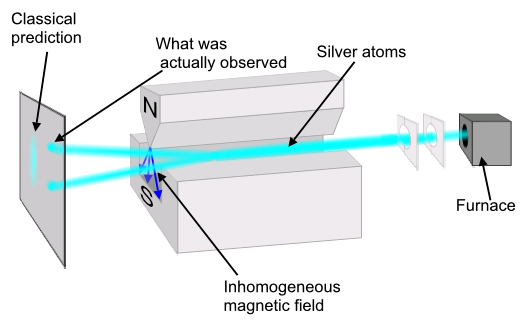
\includegraphics[width = 4.4cm]{./../Pictures/fig8_3.png}
	\figcaption{Stern-Gerlach实验图示。实验在最初使用银原子,它的自旋仅由原子轨道最外层电子的自旋决定,因此实验结果与电子相同。一束粒子流通过不均匀磁场,对于经典类型的轨道角动量,粒子在磁场偏离形成连续分布。然而实验只观测到两种偏离,即粒子流经磁场后只分为两束,一束为自旋$\frac{1}{2}$,另一束为$-\frac{1}{2}$。 图片作者为Theresa Knott (Wikimedia Commons)distributed under a CC BY-SA 3.0 license: \url{http://creativecommons.org/
	licenses/by-sa/3.0/deed.en} 图片地址:\url{https://upload.wikimedia.org/wikipedia/commons/e/ee/Stern-Gerlach_experiment_svg.svg} }
}


算符$\hat{S}_3$的显式形式为
\begin{equation}
	\hat{S}_3 = \frac{\sigma_3}{2} =
		\begin{pmatrix}
			\frac{1}{2} & 0 \\
			0 & -\frac{1}{2}
		\end{pmatrix}
\label{equ8.46}
\end{equation}
相应的本征态为
\begin{equation}
	v_{\frac{1}{2}} =
		\begin{pmatrix}
			1 \\ 0
		\end{pmatrix}
	\quad
	v_{-\frac{1}{2}} =
		\begin{pmatrix}
			0 \\ 1
		\end{pmatrix}
\label{equ8.47}
\end{equation}
相应的本征值分别为$\frac{1}{2}, -\frac{1}{2}$。这意味着旋量\mpar{回顾:旋量是坐标变换下按照Lorentz群的$(\frac{1}{2}, 0)$表示或$(0, \frac{1}{2})$表示或$(\frac{1}{2}, 0) \oplus (0, \frac{1}{2})$表示变换的量。}描述的粒子的自旋为$\frac{1}{2}$,方向与坐标轴平行或反向。自旋$\frac{1}{2}$表示的名字正是来源于此。量子理论诠释为自旋只能取$\frac{1}{2}$或$-\frac{1}{2}$。\ref{sec4.5.4}节讲过,自旋与轨道角动量有些相似,并且它们源自旋转不变性。从上面的讨论可见自旋的观测结果有着奇特的性质,该性质最著名的实验验证是 Stern-Gerlach 实验(见图8.3)。

自旋的这一性质在任意方向都成立。测量自旋的$x-, y-$或$z-$分量的结果只有$\frac{1}{2}$或$-\frac{1}{2}$.

下面看一个用量子理论描述自旋测量的例子。前面说过,自旋算符(以$z$分量为例)的显式形式为(\eqref{equ5.4}式):
\begin{equation}
\label{equ8.48}
	\hat{S}_z = \frac{1}{2} \sigma_3 =
		\begin{pmatrix}
			\frac{1}{2} & 0 \\
			0 & -\frac{1}{2}
		\end{pmatrix}
\end{equation}
本征态为$|\frac{1}{2}\rangle_z \hat{=} \begin{pmatrix} 1 \\ 0 \end{pmatrix}$以及$|-\frac{1}{2}\rangle_z \hat{=} \begin{pmatrix} 0 \\ 1 \end{pmatrix}$,其中下标$z$表示与$\hat{S}_z$有关。一般的旋量并非本征态自旋,而是它们的线性叠加,即$|X\rangle = a |\frac{1}{2}\rangle_z + b |-\frac{1}{2}\rangle_z$. 系数决定特定状态。如果观测一束粒子流的$z$分量,并“过滤”掉自旋$-\frac{1}{2}$的部分\footnote{这可以用前面提到的Stern-Gerlach实验装置完成。},则筛选后的粒子自旋状态的系数$b = 0, a = 1$,在筛选之前,状态为$a = b = \frac{1}{\sqrt{2}}$,这意味着两种自旋的概率\mpar{系数$a, b$与概率幅直接相关,下面就会看到。}相等均为$\frac{1}{2}$。先后测量粒子自旋在不同方向分量(例如,先测量$S_z$再测量$S_x$)的结果十分有趣。即使把所有自旋$-\frac{1}{2}$粒子都筛选出去,其余的仍有$S_x = -\frac{1}{2}$的粒子。

自旋算符$\hat{S}_z$作用于态矢意味着测量自旋的$z$分量。对于一般状态$|X \rangle$,测量结果为$\frac{1}{2}$或$-\frac{1}{2}$的概率由系数$a, b$决定。如果测量结果为$-\frac{1}{2}$的概率已知,则相应的概率幅为
\begin{equation}
	\ _z\langle -\frac{1}{2} || X \rangle = a\underbrace{ \ _z\langle -\frac{1}{2} || \frac{1}{2} \rangle_z }_{ = 0} + b \underbrace{ \ _z \langle -\frac{1}{2} || -\frac{1}{2} \rangle_z }_{=1} = b.
\label{equ8.49}
\end{equation}
因此测量自旋$z$分量所得结果为$-\frac{1}{2}$的概率为$P_{z = -\frac{1}{2}} = |b|^2$. 测量其他方向的分量,例如$x$轴,即用自旋算符$\hat{S}_x$作用于态矢,$S_x$的矩阵形式为(\eqref{equ5.4}式):
\begin{equation}
	S_x =
		\begin{pmatrix}
			0 & \frac{1}{2} \\
			\frac{1}{2} & 0
		\end{pmatrix}
\label{equ8.50}
\end{equation}
它的本征值仍为$\pm \frac{1}{2}$,本征矢分别为$|\frac{1}{2} \rangle_x \hat{=} \frac{1}{\sqrt{2}} \begin{pmatrix} 1 \\ 1 \end{pmatrix}$以及$|-\frac{1}{2} \rangle_x \hat{=} \frac{1}{\sqrt{2}} \begin{pmatrix} 1 \\ -1 \end{pmatrix}$,要计算$S_x = -\frac{1}{2}$的概率,需要将$|\frac{1}{2} \rangle_z$与$|-\frac{1}{2} \rangle_z$用$|\frac{1}{2} \rangle_x, |-\frac{1}{2} \rangle_x$表示:
\begin{align}
	\underbrace{|\frac{1}{2} \rangle_z}_{\begin{pmatrix} 1 \\ 0 \end{pmatrix} } = \frac{1}{\sqrt{2}} \Big( \underbrace{ |\frac{1}{2} \rangle_x }_{ \frac{1}{\sqrt{2}} \begin{pmatrix} 1 \\ 1 \end{pmatrix} } + \underbrace{ |-\frac{1}{2} \rangle_x}_{\frac{1}{\sqrt{2}} \begin{pmatrix} 1 \\ -1 \end{pmatrix} } \Big)
\label{equ8.51} \\
	\underbrace{-|\frac{1}{2} \rangle_z}_{\begin{pmatrix} 0 \\ 1 \end{pmatrix} } = \frac{1}{\sqrt{2}} \Big( \underbrace{ |\frac{1}{2} \rangle_x }_{ \frac{1}{\sqrt{2}} \begin{pmatrix} 1 \\ 1 \end{pmatrix} } - \underbrace{ |-\frac{1}{2} \rangle_x}_{\frac{1}{\sqrt{2}} \begin{pmatrix} 1 \\ -1 \end{pmatrix} } \Big)
\label{equ8.52}
\end{align}
因此
\begin{equation}
	|X\rangle = a|\frac{1}{2}\rangle_z + b |-\frac{1}{2} \rangle_z = a\frac{1}{\sqrt{2}} \left( |\frac{1}{2} \rangle_x + |-\frac{1}{2} \rangle_x \right) + b \frac{1}{\sqrt{2}} \left( |\frac{1}{2} \rangle_x - |-\frac{1}{2} \rangle_x \right).
\label{equ8.53}
\end{equation}
测量自旋$x$分量所得结果为$-\frac{1}{2}$的概率幅为
\begin{equation}
\begin{split}
	\ _x \langle -\frac{1}{2} || X \rangle &= \ _x \langle -\frac{1}{2} | \left( a\frac{1}{\sqrt{2}} \left( |\frac{1}{2} \rangle_x + |-\frac{1}{2} \rangle_x \right) + b\frac{1}{\sqrt{2}} \left( |\frac{1}{2}_x - |-\frac{1}{2} \rangle_x \right) \right) \\
	&= \frac{a}{\sqrt{2}} - \frac{b}{\sqrt{2}}
\label{equ8.54}
\end{split}
\end{equation}
即$P_{S_x = -\frac{1}{2}} = |\frac{a}{\sqrt{2}} - \frac{b}{\sqrt{2}}|^2$.

现在考虑开头提出的问题。将所有$S_z = -\frac{1}{2}$的粒子剔除后,粒子的状态为
\begin{equation}
	|X\rangle_{z\text{方向筛选后}} = |\frac{1}{2} \rangle_z.
\label{equ8.55}
\end{equation}
即$a = 1, b = 0$,因此$S_x = -\frac{1}{2}$的概率为$P_{S_x = -\frac{1}{2}} = |\frac{1}{\sqrt{2}} - \frac{0}{\sqrt{2}}|^2 = \frac{1}{2}$. 现在再筛选掉$S_x = -\frac{1}{2}$的粒子,然后测量$S_z$,所得结果十分神奇。筛选掉所有$S_x = -\frac{1}{2}$后粒子的状态为
\begin{equation}
	|X \rangle_{x\text{方向筛选后}} = |\frac{1}{2} \rangle_x.
\label{equ8.56}
\end{equation}
要计算测量$S_z$所得结果为$-\frac{1}{2}$的概率需要将状态$|\frac{1}{2} \rangle_x$用$|\frac{1}{2} \rangle_z, |-\frac{1}{2} \rangle_z$展开:
\begin{equation}
	|X \rangle_{x\text{方向筛选后}} = \underbrace{ |\frac{1}{2} \rangle_x }_{\frac{1}{\sqrt{2}} \begin{pmatrix} 1 \\ 1 \end{pmatrix} } = \frac{1}{\sqrt{2}} \Big(  \underbrace{ |\frac{1}{2} \rangle_z}_{ \begin{pmatrix} 1 \\ 0 \end{pmatrix}} + \underbrace{|-\frac{1}{2} \rangle_z}_{\begin{pmatrix} 0 \\ 1 \end{pmatrix}} \Big)
\label{equ8.57}
\end{equation}
于是$P_{z = -\frac{1}{2}} = | \langle -\frac{1}{2} |_z |X\rangle|^2 = \frac{1}{2}$. 将上述观测结果进行总结:

\begin{itemize}
\item	初始时粒子(流)的状态任意,观测自旋的$z$分量,筛选掉所有$S_z = -\frac{1}{2}$的粒子,筛选后粒子的状态为
	\begin{equation}
		|X\rangle_{z\text{方向筛选后}} = |\frac{1}{2} \rangle_z.
	\label{equ8.58}
	\end{equation}
\item	测量筛选后粒子的自旋$z$分量的结果自然是全部为$+\frac{1}{2}$:
	\begin{align}
		\ _z\langle \frac{1}{2} || X \rangle_{z\text{方向筛选后}} &= 1.
	\label{equ8.59} \\
		\ _z \langle -\frac{1}{2} | |X \rangle_{z\text{方向筛选后}} &= 0
	\label{equ8.60}
	\end{align}
\item	再测量粒子的自旋$x$分量发现其中一半为$S_x = \frac{1}{2}$,另一半为$-\frac{1}{2}$。剔除其中所有$S_x = -\frac{1}{2}$的粒子后粒子的状态为$|X\rangle_{x\text{方向筛选后}} = |\frac{1}{2} \rangle_x$.
\item 	现在再次测量粒子的自旋$z$分量,我们得到令人吃惊的测量结果:一半粒子为$S_z = \frac{1}{2}$,另一半为$S_z = -\frac{1}{2}$. 尽管在第一步已经筛选掉所有$S_z = -\frac{1}{2}$的粒子!
\end{itemize}
关于这部分内容的精彩讨论(包括实际的观测仪器)可见Feynman物理学讲义第三卷\mpar{ Richard P. Feynman, Robert B.
Leighton, and Matthew Sands. The Feynman Lectures on Physics, Volume 3. Addison Wesley, 1st edition, 1 1971. ISBN 9780201021189}。

\section[Heisenberg 不确定性原理]{Heisenberg’s Uncertainty PrincipleHeisenberg \quad 不确定性原理}\label{sec8.6}

现在可以讨论量子力学中最奇妙的特征之一了。从上节可知,对粒子自旋$x$分量的测量会破坏已知的自旋$z$分量的信息,这一情况在量子力学的很多测量中都存在。我们可以从\mpar{我们把自旋算子和对应的有限维旋转生成元认同,其满足对易关系$[J_i,J_j]=J_i J_j -J_j J_i=i\epsilon_{ijk}J_k\ne 0 \to J_i J_j \ne J_j J_i$。 举个例子来说,描述自旋1/2的粒子应采用对应的二维表示$J_i={\sigma_i \over 2}$。} $\hat S_x \hat S_z \ne \hat S_z \hat S_x$ 出发来考察这一点,此式说明先对自旋$z$分量后对$x$分量进行测量和先对$x$分量后对$z$分量进行测量的结果是不同的。这一点并不令人惊奇,因为对$z$方向自旋进行测量后,系统应处于$\hat S_z$ 的一个本征态上,而对$x$方向自旋进行测量后,系统应处于$\hat S_x$ 的本征态上,$\hat S_z$ 和$\hat S_x$的本征态均不同,最后的结果也就不同。


上述现象可以从另一视角描述:{\bf 自旋的$x$分量与$z$分量不能同时确定!}每次测量$z$方向的自旋时,都会让$x$方向的自旋信息再次变为未知,反之亦然。这一结论对于$z$ 方向/$x$方向和$y$方向的自旋也是一样的。

你也许觉得自旋是比较奇怪的物理量,但在粒子位置和动量的测量上也发现了同样的结果。回顾一下式\eqref{equ5.3},为了方便重写一遍:
\begin{equation}
\label{equ8.16}
	[\hat p_i,\hat x_j]=\hat p_i \hat x_j - \hat x_j \hat p_j =i \delta_{ij}
\end{equation}
由上可见,对粒子位置的$x$分量进行测量,会导致之前对动量$x$分量的测量结果变得不确定。换句话说,我们不能同时{\it 足够精确地}确定粒子在同一方向上的位置与动量。注意,只有沿相同方向的位置和动量算符的对易子才不为零\mpar{Kronecher delta函数$\delta_{ij}$在$i\ne j$时为0,$i=j$时为1,其定义在附录B.5.5。},所以测量动量的$y$分量不会干扰对位置的$x$分量的测量。

每次测量动量会使位置信息变得不确定,反之亦然,这就是著名的{\bf Heisenberg 不确定原理}。同样的现象也发生在的角动量的不同分量之间,因为它们的对易子不为零。总而言之,我们可以计算任意两个物理量的对易性,如果它们不对易,它们就不能同时{\it 足够精确地}被确定。

这其实不太奇怪。量子力学使用相应对称性的生成元作为测量算符,比如说,对动量的测量等价于平移生成元的作用\mpar{复习:系统的平移不变性导出动量守恒定律。},这一生成元将我们的系统平移了一小点,所以粒子的位置也被改变了。真正令人惊奇的是大自然就是这么运作的,许多年来有很多实验验证Heisenberg不确定原理,它们都证明了这个原理的正确性。



\section[对几种诠释的评议]{Comments on Interpretations \quad 对几种诠释的评议}\label{sec8.7}
本章采用的都是量子力学的标准诠释与通用符号,然而还有其他同样有效的体系。例如,就结果而言,Feynman路径积分体系\mpar{这方面内容可参考Richard P. Feynman and Albert R. Hibbs. {\it Quantum Mechanics and Path Integrals}: Emended Edition. Dover Publications, emended editon edition, 7\ 2010. ISBN 9780486477220}与本章描述的波动力学完全等价。但二者的计算过程相当不同。在路径积分体系中计算粒子从点$a$到$b$的概率,需要将从$a$到$b$的所有可能的路径叠加。尽管听起来很奇怪,但是可以证明它的计算结果和波动力学相同。Freeman Dyson曾经讲过关于路径积分的一个故事\mpar{Harry Woolf, editor. {\it Some Strangeness in the Proportion}. Addison-Wesley, 1st edition, 2\ 1981. ISBN 9780201099249}:

\begin{quote}
Dick Feynman向我讲述他量子力学“历史态叠加”的新理论。 "The electron does anything it likes," he said. "It just goes in any direction at any speed, forward or backward in time, however it likes, and then you add up the amplitudes and it gives you the wavefunction."
我对他说:“你疯啦。”但实际上他没疯。
\end{quote}

量子力学基本方程的另一种基本诠释(比起路径积分更加偏离主流)是Bohm诠释。它的出发点是在Schrödinger方程中加入拟设项$R \mathrm{e}^{St}$. 方程的实部与虚部构成两个方程,其中一个可以类比为经典力学中的Hamilton-Jacobi方程(有附加项,附加项可以解释为与量子效应有关的额外势能),进一步的计算就与经典力学非常相似。对额外势求梯度得到新的力,可以带入Newton的经典方程$F = ma$中。因此在Bohm诠释中仍然存在经典的粒子轨道。据我所知,Bohm诠释的计算结果与标准非相对论量子力学的计算结果相同。然而由于额外势的非定域性使得它不受欢迎。


\section*{阅读建议}
\begin{itemize}
\item {\bf Richard P. Feynman - The Feynman Lectures on Physics, Vol. 3}\mpar{Richard P. Feynman, Robert B. Leighton, and Matthew Sands. {\it The Feynman Lectures on Physics, Volume 3}. Addison Wesley, 1st edition, 1 1971. ISBN 9780201021189} 是量子力学入门的出色教材。量子力学的大部分概念都在此书中有更清楚的解释。
\item {\bf  David J. Griffiths - Introduction to Quantum Mechanics}\mpar{ David J. Griffiths. Introduction to Quantum Mechanics. Pearson Pren-
tice Hall, 2nd edition, 4 2004. ISBN 9780131118928}
是非常易读的、具有启发性的教材。
\item {\bf  J. J. Sakurai - Modern Quantum Mechanics}\mpar{ {\it J. J. Sakurai. Modern Quantum Mechanaics}. Addison Wesley, 1st edition, 9 1993. ISBN 9780201539295}是一本精彩著作,它提供了量子力学的独特视角。
\item {\bf Paul A. M. Dirac - Lectures on Quantum Mechanics}\mpar{Paul A. M. Dirac and Physics. {\it Lectures on Quantum Mechanics.} Dover Publications, 1st edition, 3 2001. ISBN 9780486417134}是量子力学的原始文献之一。尽管古老,但时至今日它的评价依然很高,因为阅读量子力学创始人的思想是非常具有启示意义。
\item Dirac旋量的分量意义的详细诠释可参考附录8.8。
\end{itemize}


\section[附录:Dirac旋量分量的诠释]{Appendix: Interpretation of the Dirac Spinor Components \quad 附录:Dirac旋量分量的诠释}\label{sec8.8}
{\it 在接下来的附录中,$\mathbf{u}, \mathbf{v}$表示Dirac旋量里面的二分量对象,$u, v$表示四分量对象。例如,$u_1, u_2$描述两个不同的四分量对象。一个一般的四分量对象$u$相应的二分量对象记作$\mathbf{u}_1, \mathbf{u}_2$,即$u = \begin{pmatrix} \mathbf{u}_1 \\ \mathbf{u}_2 \end{pmatrix}$.
}

目前我们对Dirac旋量中的两个Weyl旋量的认识还比较模糊。它们究竟代表什么?应该被诠释成什么?此外,Dirac旋量里的Weyl旋量也具有两个分量,这该怎么解释?下面就来讨论。

{\it 简言之:}

\begin{itemize}
\item Dirac旋量$\psi \begin{pmatrix} \chi_L \\ \xi_R \end{pmatrix}$中的两个Weyl旋量$\chi_L, \xi_R$描述“不同的粒子”。然而惯例上仍然称它们是相同的粒子,只是手征性不同,例如对电子而言:
\begin{itemize}
\item[-] $\chi_L$描述左手电子(left-chiral electron)。
\item[-] $\xi_R$描述右手电子(right-chiral electron)。
\end{itemize}
实际上它们是十分不同的粒子或场\mpar{它们由不同的量子数标记,因此实验性质相当不同!},因为它们不能由宇称变换或电荷共轭相联系。因此采用不同的符号$\chi, \xi$表示它们。当然它们存在某些关系,不然为啥写在同一个旋量里呢… 这一点稍后再说。

\item Weyl旋量的两个分量描述粒子不同的自旋构型\mpar{自旋构型在\ref{sec8.5.5}节讨论。复习一下,自旋与普通角动量的测量方法相似,只是例如自旋$\frac{1}{2}$粒子自旋所有方向分量的测量结果只能是$\frac{1}{2}$或$-\frac{1}{2}$,它们通常称作{\bf 自旋向上}与{\bf 自旋向下}。}。
\begin{itemize}
\item[-] 正比于$\begin{pmatrix} 1 \\ 0 \end{pmatrix}$的Weyl旋量描述{\bf 自旋向上}的粒子。
\item[-] 正比于$\begin{pmatrix} 0 \\ 1 \end{pmatrix}$的Weyl旋量描述{\bf 自旋向下}的粒子。
\item[-] 其他Weyl旋量仅仅是自旋向上/向下状态的叠加。
\end{itemize}
\end{itemize}

{\it 下面进行详细推导:}

弱相互作用和宇称破缺使得我们明白了左手手性和右手手性是截然不同的粒子这一重要观点。左手手性的粒子携带弱荷(同位旋),因此通过弱力来相互作用。右手手性的粒子则不携带,因此不相互作用,我们在\ref{sec7.7.1}中有过解释。

我们自然界中的每一个粒子都有它对应的反粒子,而其反粒子的描述就是通过对粒子的荷进行共轭操作。荷的共轭操作会翻转所有的粒子的标签,当然包括同位旋。我们可以看看,对应于电子,其对应什么样的粒子。我们有
\begin{itemize}
\item 一个左手手性的{\it 电子}$\chi_L$,同位旋$-\frac{1}{2}$,带电$-e$,处于双重态。
\item 一个右手手性的{\it 反-左手手性电子}$(\chi_L)^c=\chi_R$,将有同位旋$\frac{1}{2}$,电荷$+e$,也同样是处于双重态。这种特性不会因为荷共轭就消失。这可能看起来有点迷茫,但是到现在为止我们只讨论粒子\footnote{而不是反粒子,切记切记}间弱力带来的耦合。右手反粒子也会被弱相互作用耦合。
\item 右手{\it 电子}$\xi_R$,同位旋$0$,电荷$-e$。
\item 左手{\it 反-右手手性电子}$(\xi_R)^c=\xi_L$,同位旋$0$,电荷$+e$。
\end{itemize}

因此,当讨论电子的时候,我们实际上有{\bf 四}种不同的需要考虑的``东西''。因为他们都是不同的粒子,我们实际上需要给他们不同的名字!一般我们只会说两种:电子和正电子,我们马上会看到这意味着什么。

{\it 我们接下来的讨论仅限于问题中的粒子静止的参考系。在其他的参考系中,这些讨论是类似的,但是会有琐碎的细节。}

Dirac旋量和其荷共轭与这四种粒子直接相关。{\bf 物理的电子}和{\bf 物理的正电子}一般被认为是DIrac方程的解。Dirac方程是运动方程,也就是决定粒子的动力学的方程,其解为DIrac旋量的时间演化。我们需要求出来我们的粒子的时间演化,这就需要我们同时考虑这两种粒子。

在附录,\ref{sec8.9}节中我们可以看到严格的推导。我们这里给出结论。Dirac方程有四个线性无关的解,其中两个有形式
\begin{align}
\psi_i=\left(\begin{matrix}\text{u}_i\\\text{u}_i\end{matrix}\right)
\end{align}
比如\mpar{这实际上是一种基的选取。任何选取只需要线性无关就可以。}$\text{u}_1=\left(\begin{matrix}1\\0\end{matrix}\right)e^{-imt}$和$\text{u}_2=\left(\begin{matrix}0\\1\end{matrix}\right)e^{-imt}$,而另外两个有形式
\begin{align}
\bar{\psi}_i=\left(\begin{matrix}-\text{v}_i\\\text{v}_i\end{matrix}\right)
\end{align}
比如$\text{v}_1=\left(\begin{matrix}1\\0\end{matrix}\right)e^{+imt}$和$\text{v}_2=\left(\begin{matrix}0\\1\end{matrix}\right)e^{+imt}$。

Dirac方程告诉我们两个粒子的自旋由Dirac旋量里面的上下Weyl旋量来描述。不仅如此,他们的时间依赖必须一样。这些解就是我们通常认为的不同自旋的{\bf 物理电子}和{\bf 物理正电子}\mpar{注意这些解彼此之间的荷共轭。利用荷共轭算符来仔细计算:$\psi_1^c=i\gamma_2\psi_1^*$,因此$(\psi_1)^c=\bar{\psi}_2$,而$(\psi_2)^c=\bar{\psi}_1$。}。

\begin{itemize}
\item $\psi_1$是自旋向上的电子
\item $\psi_2$是自旋向下的电子
\item $\bar{\psi}_1$是自旋向上的电子
\item $\bar{\psi}_2$是自旋向下的电子
\end{itemize}

我们可以看到一个物理电子有一个左手(上面的两分量)和右手(下面的两分量)成分。一个物理电子的左右手成分的自旋、时间依赖必须是一样的。就如上面所讨论的,左手和右手成分的行为是非常不一样的,因为他们有不同的弱荷!而为了描述他们的动力学,物理电子必须同时有这两个成分。

注意这些解并不意味着我们用来描述物理电子用的是严格的上和下分量。只需要他们的自旋和时间依赖必须一样。上部分仍然是双重态,而下部分则不是。上部分按照$SU(2)$变化而下部分不是。用前面的符号来看的话,我们有
\begin{align}
\text{物理电子}=\left(\begin{matrix}\chi_L\\\xi_R\end{matrix}\right)\propto\left(\begin{matrix}\text{u}\\\text{u}\end{matrix}\right)
\end{align}
这并不说明$\chi_L=\xi_R$。Weyl旋量$\chi_L$是有同位旋的双重态,而由$\xi_R$描述的粒子则没有同位旋。不仅如此,我们也知道了Dirac旋量里面的上和下Weyl旋量在Lorentz推动下是不一样变化的。因此,我们使用不同的记号是非常有必要的。换句话说,左手电子$\chi_L$带一个$SU(2)$指标,因为$\chi_L$按照$SU(2)$双重态的一部分来变换。$\xi_R$则没有指标,按照$SU(2)$单重态来变化呢。

一样的 ,我们有
\begin{align}
\text{物理正电子}=\left(\begin{matrix}-\xi_L\\\chi_R\end{matrix}\right)\propto\left(\begin{matrix}-\text{v}\\\text{v}\end{matrix}\right)
\end{align}
我们可以通过荷共轭看到\mpar{见第\ref{sec7.1.5}节,并利用\eqref{equ6.13}定义的矩阵的精确形式:$\gamma_2=\left(\begin{matrix}0&\bar{\sigma_2}\\\sigma_2&0\end{matrix}\right)=\left(\begin{matrix}0&-{\sigma_2}\\\sigma_2&0\end{matrix}\right)$。}
\begin{align}
\begin{split}
(\text{物理电子})^c&=i\gamma_2\left(\begin{matrix}\xi_L\\\chi_R\end{matrix}\right)^*=\left(\begin{matrix}-\chi_L\\\xi_R\end{matrix}\right)\propto i\gamma_2\left(\begin{matrix}\text{u}\\\text{u}\end{matrix}\right)^*=\left(\begin{matrix}-\text{u}^c\\\text{u}^c\end{matrix}\right)\\
&=\text{物理正电子}
\end{split}
\end{align}

这告诉我们我们自然界中观测到的物理电子实际上大部分时候都是两种粒子的叠加:携带同位旋的左手电子和无同位旋的右手电子!一样的我们知道,物理正电子也是由携带同位旋的反-左手电子和无同位旋的反-右手粒子的混合。

Dirac方程的解则告诉我们粒子如何进行时间演化。比如说我们考虑在一个弱相互作用下出现的一个自旋向上的电子,然后它如何进行时间演化呢?首先他是一个纯的左手电子,可以写为
\begin{align}
e_L^\uparrow=\left(\begin{matrix}1\\0\\0\\0\end{matrix}\right)
\end{align}
而它并不是Dirac方程的解,因此,为了得到它的时间演化,我们可以用Dirac方程的解展开:
\begin{align}
e_L^\uparrow=\left(\begin{matrix}1\\0\\0\\0\end{matrix}\right)=\frac{1}{2}\left(\left(\begin{matrix}1\\0\\1\\0\end{matrix}\right)-\left(\begin{matrix}-1\\0\\1\\0\end{matrix}\right)\right)=\Psi_1(t=0)-\bar{\Psi}_1(t=0)
\end{align}
我们知道$\Psi_1$和$\bar{\Psi}_1$如何时间演化
\begin{align}
\Psi_1(t)-\bar{\Psi}_1(t)=\to\frac{1}{2}\left(\left(\begin{matrix}1\\0\\1\\0\end{matrix}\right)e^{-imt}-\left(\begin{matrix}-1\\0\\1\\0\end{matrix}\right)e^{imt}\right)
\end{align}
对于$t=0$,这就是左手态,但是演化了一段时间,比如$t=\frac{\pi}{2m}$之后,我们有
\begin{align}
\to\frac{1}{2}\left(\left(\begin{matrix}1\\0\\1\\0\end{matrix}\right)\underbrace{e^{-i\frac{\pi}{2}}}_{=-i}-\left(\begin{matrix}-1\\0\\1\\0\end{matrix}\right)\underbrace{e^{i\frac{\pi}{2}}}_{=i}\right)=-i\left(\begin{matrix}0\\0\\1\\0\end{matrix}\right)=-ie_R^\uparrow
\end{align}
这描述了一个自旋向上的右手电子!这里我们了解到,随着时间演化,左手粒子会变成右手粒子,反之亦然。为了描述电子的演化,我们必须有$e_L$和$e_R$,这也就是我们把它们在一起写成Dirac旋量的原因。对正电子亦然。

记得两种不同的粒子$e_L$,$e_R$有不同的弱荷,即同位旋,而时间演化可以使二者互相转换。大多数时候它们都是两种的混合物,而不是确切的处于某个本征态。同位旋和手性因此在时间演化中就不守恒。

我们现在可以看到Dirac旋量的符号是必须的,因为我们有一个封闭的将本节开始提到的四种粒子中任意两种联系起来的动力学行为。手性和同位旋在传播过程中也就不守恒了。可以发现,不同时间的电子有的时候处于左手态,有的时候也会处于右手态。




\section[附录:解Dirac 方程]{Appendix: Solving the Dirac Equation 附录:解Dirac 方程}\label{sec8.9}
{\it 和上节一样,我们把Dirac自旋量中的二分量量记做{\rm u}和{\rm v},把四分量量记做$u$和$v$。也就是说例如$u_1,u_2$的记号代表的是四分量量,在不特别区分这些量的时候我们只写$u$。同时${\rm u_1}$和${\rm u_2}$是这个四分量量中的两个二分量量:$u=\pmm \rm u_1 \\ \rm u_2 \pmme $}。
\par
本附录中我们将在{\it 手性基底}上解{\it 静止参考系}下的Dirac方程。其他任意参考系的解能够通过本节解做伪转动变换得到。除了我们在上一节的讨论,我们在第六章讨论量子场论的时候也会用到这些解。\par
Dirac方程为:
\begin{equation}
(i\partial_\mu \gamma^\mu -m)\psi=0
\end{equation}
我们考虑其平面波解,设$\Psi=ue^{-ipx}$,其中$u$是一四分量量,因为矩阵$\gamma_\mu$是$4 \times 4$的。在静止参考系中,三维动量$\vec{p}=0$,指数项因此变为$-ipx=-i(p_0x_0-\vec{p}\vec{x})=-ip_0x_0$。现在使用我们本章初推导得到的相对论能量动量关系$E=\sqrt{|\vec{p}|^2+m^2}$,已知$p_0=E$和$x_0=t$,我们得到$-ipx=-iEt=-i\sqrt{|\vec{p}|^2+m^2}t=-imt$。把此式带入到Dirac方程中:
\begin{equation}
\begin{split}
&(i\partial_\mu\gamma^\mu-m)ue^{-imt}=0\\
&\to (i(\partial_0\gamma^0-\partial_i\gamma_i)-m)ue^{-imt}=0\\
&\to (i(-im)\gamma^0-m)ue^{-imt}=0\\
&\to (m\gamma^0-m)u=0\\
&\to (\pmm 0 & 1 \\ 1 & 0 \pmme -\pmm 1 & 0 \\ 0 & 1 \pmme)u=0\\
&\to \pmm -1 & 1 \\ 1 & -1 \pmme \pmm \rm u_1 \\ \rm u_2 \pmme =0\\
&\to \pmm \rm -u_1+u_2 \\ \rm u_1-u_2 \pmme =0
\end{split}
\end{equation}
注意这里矩阵中的1实际上代表的是$2 \times 2$的单位矩阵,所以$\rm u_1$和$\rm u_2$是二分量量。我们看出我们假设的平面波解在$\rm u_1 =u_2$的条件下符合方程,由此我们找到了Dirac方程两个线性独立的解:
\begin{equation}
\Psi_1=\pmm 1\\0\\1\\0 \pmme e^{-imt},~~~\Psi_2=\pmm 0\\1\\0\\1 \pmme e^{-imt}
\end{equation}
我们可以通过设$\tilde \Psi =ve^{ipx}$来得到另外两个解,在静止参考系下这一解形式化为$\tilde \Psi=ve^{imt}$,带入方程得
\begin{equation}
\begin{split}
&(i\partial_\mu\gamma^\mu-m)ve^{imt}=0\\
&\to (-m\gamma^0-m)v=0\\
&\to \pmm -1 & -1 \\ -1 & -1 \pmme \pmm \rm v_1 \\ \rm v_2 \pmme =0\\
&\to \pmm \rm -v_1-v_2 \\ \rm -v_1-v_2 \pmme =0
\end{split}
\end{equation}
我们由此得到时间依赖为$e^{imt}$的两个解,其满足$\rm -v_1=v_2$的条件。此时两个线性独立的解为:
\begin{equation}
\tilde \Psi_1=\pmm 1\\0\\-1\\0 \pmme e^{imt},~~~\tilde \Psi_2=\pmm 0\\1\\0\\-1 \pmme e^{imt}
\end{equation}



\section[附录:Dirac 旋量的不同的基]{Appendix: Dirac Spinors in Different Bases 附录:Dirac 旋量的不同的基}\label{sec8.10}

在拉格朗日量中,Dirac 旋量$\psi$总是和矩阵$\gamma_\mu$组合出现。
这个特性可以通过转换到一个不同的基来简化计算。
这种简化之所以行得通,是因为对于任意的可逆矩阵$N$,我们都可以通过在$\psi$和$\gamma_\mu$之间插入形如$1=N^{-1}N$的项来重新定义两者。
\begin{align}
  \partial_\mu\bar{\psi}\gamma_\mu\psi = \partial_\mu\bar{\psi}\underbrace{N^{-1}N}_{\mathclap{=1}}\gamma_\mu\underbrace{N^{-1}N}_{\mathclap{=1}}\psi = \partial_\mu\underbrace{\bar{\psi}N^{-1}}_{\mathclap{\equiv\bar{\psi}'}}\underbrace{N\gamma_\mu N^{-1}}_{\mathclap{\equiv\gamma'_\mu}}\underbrace{N\psi}_{\mathclap{\equiv\psi'}}
\end{align}
目前为止我们在本书中使用的基被称为手性基或者 Weyl 基。
而习惯上 Dirac 方程的求解中用的是另一种基,被称为质量基或者 Dirac 基。
在我们目前为止使用的手性或 Weyl 基中,Dirac 拉格朗日量
\begin{align}
  \mathcal{L}_D=i\chi_L^\dagger\sigma^\mu\partial_\mu \chi_L+i\xi_R^\dagger\bar{\sigma}^\mu\partial_\mu \xi_R-m\chi_L^\dagger\xi_R-m\xi_R^\dagger\chi_L
\end{align}
具有非对角的质量项——也就是混合了不同的态的质量项。
我们可以利用选择基的自由度来找到一组使得质量项对角的基,并将之称为质量基。

这意味着我们想要形如$\psi^\dagger m\psi$的质量项,其中$m=\begin{pmatrix}m_1&0\\0&m_2\end{pmatrix}$,
于是我们就得到了质量项的形式是
\begin{align}
  \bar{\psi}'M'\psi'=(\psi')^\dagger%此处原书中不带',应为印刷错误,但是勘误表中没有。带‘应为正确形式,故改正并说明。
  \gamma'_0M'\psi'=\begin{pmatrix}u'\\v'\end{pmatrix}^\dagger\begin{pmatrix}m_1&0\\0&m_2\end{pmatrix}
  \begin{pmatrix}u'\\v'\end{pmatrix}=(u')^\dagger m_1u'+(v')^\dagger m_2v',
\end{align}
而我们正在处理的是
\begin{align}
  \bar{\psi}M\psi=\psi^\dagger\gamma_0M\psi=\begin{pmatrix}\chi_L\\\xi_R\end{pmatrix}^\dagger\begin{pmatrix}0&m\\m&0\end{pmatrix}
  \begin{pmatrix}\chi_L\\\xi_R\end{pmatrix}=m\chi_L^\dagger\xi_R+m\xi_R^\dagger\chi_L.
\end{align}
我们目前为止一直使用的后一个基很容易体现出手性,然而质量基下的 Dirac 旋量会更容易和物理中的传播粒子建立联系。

为了得到第二个形式和第一个形式间的关系,我们需要把矩阵$M=\begin{pmatrix}0&m\\m&0\end{pmatrix}=m\begin{pmatrix}0&1\\1&0\end{pmatrix}$对角化。
这个矩阵的对角化可以通过矩阵$N=\frac{1}{\sqrt{2}}\begin{pmatrix}-1&1\\1&1\end{pmatrix}$来实现,
也就是说
\begin{align}
  N^{-1}\underbrace{\begin{pmatrix}-m&0\\0&m\end{pmatrix}}_{\mathclap{\equiv M'}}N=M
\end{align}
\begin{align}
  \rightarrow m\frac{1}{\sqrt{2}}\begin{pmatrix}-1&1\\1&1\end{pmatrix}^-1\begin{pmatrix}-1&0\\0&1\end{pmatrix}\frac{1}{\sqrt{2}}
  \begin{pmatrix}-1&1\\1&1\end{pmatrix}=m\begin{pmatrix}0&1\\1&0\end{pmatrix}
\end{align}
于是我们就可以相应地重新定义 Dirac 旋量
\begin{align}
\begin{split}
  \bar{\psi}M\psi=&\bar{\psi}\underbrace{NN^{-1}}_{\mathclap{=-1}}M\underbrace{NN^{-1}}_{\mathclap{=-1}}\psi\\
  =&\underbrace{\bar{\psi}N}_{\mathclap{\equiv\bar{\psi}'}}
  \underbrace{N^{-1}MN}_{\mathclap{\equiv M'}}\underbrace{N^{-1}\psi}_{\mathclap{\equiv\psi'}}\\
  =&\bar{\psi}'M'\psi'
  \end{split}
\end{align}

观察一下在这个基下的手性投影算符$P_L=\frac{1-\gamma_5}{2}$是很有帮助的。
因此我们需要得出相应的$\gamma_5$矩阵
\begin{align}
\begin{split}
  \bar{\gamma}_5=N^{-1}\gamma_5N=&\frac{1}{\sqrt{2}}\begin{pmatrix}1&1\\1&-1\end{pmatrix}\begin{pmatrix}1&0\\0&-1\end{pmatrix}
  \frac{1}{\sqrt{2}}\begin{pmatrix}1&1\\1&-1\end{pmatrix}\\
  =&\frac{1}{2}\begin{pmatrix}1&1\\1&-1\end{pmatrix}\begin{pmatrix}1&1\\-1&1\end{pmatrix}\\
  =&\begin{pmatrix}0&1\\1&0\end{pmatrix}
\end{split}
\end{align}
与此对应的本征向量是$\frac{1}{\sqrt{2}}\begin{pmatrix}1\\-1\end{pmatrix}$和$\frac{1}{\sqrt{2}}\begin{pmatrix}1\\1\end{pmatrix}$。
这表示手性本征态现在由具有上下分量的 Dirac 旋量描述,
例如,左手态在这个基下的形式就是$\frac{1}{\sqrt{2}}\begin{pmatrix}1\\-1\end{pmatrix}$
相比之下,在手性基下$\gamma_5$是对角的,左手本征态由只有上分量的 Dirac 旋量$\psi_L=\begin{pmatrix}\chi_L\\0\end{pmatrix}$给出,
右手本征态则由只有下分量的 Dirac 旋量$\psi_R=\begin{pmatrix}0\\\xi_R\end{pmatrix}$给出。

在这个基下手性投影算符写成
\begin{align}
  P_L=\frac{1-\gamma_5}{2}=\frac{1}{2}\begin{pmatrix}1&-1\\-1&1\end{pmatrix}
\end{align}

\subsection[质量基下 Dirac 方程的解]{Solutions of the Dirac Equation in the Mass Basis 质量基下 Dirac 方程的解}\label{sec8.10.1}

我们可以求解质量基下的 Dirac 方程
\begin{align}
  (i\gamma_\mu\partial^\mu-m)\Psi=0
\end{align}
通过假设$\psi=ue^{-ipx}$,可以导出
\[(\gamma_\mu p^\mu-m)ue^{-ipx}=0\]
\[\rightarrow(\gamma_\mu p^\mu-m)u=0.\]
等价地,我们可以假设$\psi=ve^{-ipx}$导出
\[(-\gamma_\mu p^\mu-m)ve^{ipx}=0\]
\[\rightarrow(-\gamma_\mu p^\mu-m)v=0.\]
类似在手性基中的解,我们这里也在静止坐标系中求解,也就是$\vec{p}=0$。
我们做这样的选择之所以可行,是因为物理规律在所有参照系中都是相同的,所以我们可以选择最符合我们需求的一个。
在这个参照系中,由于$p_i=0$,所以我们有
\[\rightarrow(\gamma_0p^0-m)u=0\]
\[\rightarrow(-\gamma_0p^0-m)v=0.\]
此外还有$p_0=E$,并且我们可以使用我们在本章开头(式\eqref{equ8.2})推导的相对论能-动量关系。
在静止参照系中我们有$E=\sqrt{(p_i)^2+m^2}=m$。
现在我们可以利用上面给出的矩阵$N$和$\gamma'_0=N^{-1}\gamma_0N$计算出$\gamma_0$在质量基或 Dirac 基中的精确形式。
要记得在$m$中我们还包含着一个单位矩阵,因此
\[\rightarrow\left(\begin{pmatrix}1&0\\0&-1\end{pmatrix}m-m\begin{pmatrix}1&0\\0&1\end{pmatrix}\right)u=0\]
\[\rightarrow\left(-\begin{pmatrix}1&0\\0&-1\end{pmatrix}m-m\begin{pmatrix}1&0\\0&1\end{pmatrix}\right)v=0.\]
\[\rightarrow\begin{pmatrix}0&0\\0&-2\end{pmatrix}u=0\]
\[\rightarrow\begin{pmatrix}-2&0\\0&0\end{pmatrix}v=0.\]
要记得每个 Dirac 旋量都包含两个二分量的变量,我们可以推出$u$的下面的二分量变量和$v$的上面的二分量变量必定是0:
\[\rightarrow\begin{pmatrix}0&0\\0&-2\end{pmatrix}\begin{pmatrix}u_1\\u_2\end{pmatrix}=\begin{pmatrix}0\\-2u_2\end{pmatrix}=0\rightarrow u_2=0\]
\[\rightarrow\begin{pmatrix}-2&0\\0&0\end{pmatrix}\begin{pmatrix}v_1\\v_2\end{pmatrix}=\begin{pmatrix}-2v_1\\0\end{pmatrix}=0\rightarrow v_1=0.\]

我们可以看到在这个基下物理的传播粒子(也就是 Dirac 方程的解)可以用只含有上分量的旋量描述,而等价地对于反粒子则只含有下分量。
从而我们可以再次得到四个线性独立的解
\begin{align}
\Psi'_1=\begin{pmatrix}1\\0\\0\\0\end{pmatrix}e^{-imt}~~~~~~\Psi'_2=\begin{pmatrix}0\\1\\0\\0\end{pmatrix}e^{-imt}
\end{align}
和

\begin{align}
\Psi'_3=\begin{pmatrix}0\\0\\1\\0\end{pmatrix}e^{imt}~~~~~~\Psi'_4=\begin{pmatrix}0\\0\\0\\1\end{pmatrix}e^{imt}
\end{align}

在这个参照系中这个基下的一般解,可以写成线性组合的形式
\begin{align}
\psi=ue^{-ipx}+ve^{ipx}=\begin{pmatrix}u_1\\0\end{pmatrix}e^{-ipx}+\begin{pmatrix}0\\v_1\end{pmatrix}e^{ipx}
\end{align}
并且我们可以通过将这个解做一个 Lorentz 推动变换得到任意一个参照系中的解。
此外,最一般的解是所有动量和自旋态\mpar{注意 Weyl 旋量的两个分量代表不同的自旋态。}的解的叠加

\begin{align}
\Psi=\sum_r\sqrt{\frac{m}{(2\pi)^3}}\int\frac{d^3p}{\sqrt{E_p}}\left(c_r(p)u_r(p)e^{-ipx}+d^\dagger_r(p)v_r(p)e^{+ipx}\right)
\end{align}
